% bei Standalone in documentclass noch:
% \RequirePackage{luatex85}

\documentclass[captions=tableheading, titlepage= firstiscover, parskip = half , bibliography=totoc]{scrartcl}
%paper = a5 für andere optinen
% titlepage= firstiscover
% bibliography=totoc für bibdateien
% parskip=half  Veränderung um Absätze zu verbessern

\usepackage{scrhack} % nach \documentclass
\usepackage[aux]{rerunfilecheck}
\usepackage{polyglossia}
\usepackage[style=numeric, backend=biber]{biblatex} % mit [style = alphabetic oder numeric] nach polyglossia
\addbibresource{lit.bib}
\setmainlanguage{german}

\usepackage[autostyle]{csquotes}
\usepackage{amsmath} % unverzichtbare Mathe-Befehle
\usepackage{amssymb} % viele Mathe-Symbole
\usepackage{mathtools} % Erweiterungen für amsmath
\usepackage{fontspec} % nach amssymb
% muss ins document: \usefonttheme{professionalfonts} % für Beamer Präsentationen
\usepackage{longtable}

\usepackage[
math-style=ISO,    % \
bold-style=ISO,    % |
sans-style=italic, % | ISO-Standard folgen
nabla=upright,     % |
partial=upright,   % /
]{unicode-math} % "Does exactly what it says on the tin."
\setmathfont{Latin Modern Math}
% \setmathfont{Tex Gyre Pagella Math} % alternativ

\usepackage[
% die folgenden 3 nur einschalten bei documenten
locale=DE,
separate-uncertainty=true, % Immer Fehler mit ±
per-mode=symbol-or-fraction, % m/s im Text, sonst \frac
]{siunitx}

% alternativ:
% per-mode=reciprocal, % m s^{-1}
% output-decimal-marker=., % . statt , für Dezimalzahlen

\usepackage[
version=4,
math-greek=default,
text-greek=default,
]{mhchem}

\usepackage[section, below]{placeins}
\usepackage{caption} % Captions schöner machen
\usepackage{graphicx}
\usepackage{grffile}
\usepackage{subcaption}

% \usepackage{showframe} Wenn man die Ramen sehen will

\usepackage{float}
\floatplacement{figure}{htbp}
\floatplacement{table}{htbp}

\usepackage{mhchem} %chemische Symbole Beispiel: \ce{^{227}_{90}Th+}


\usepackage{booktabs}

 \usepackage{microtype}
 \usepackage{xfrac}

 \usepackage{expl3}
 \usepackage{xparse}

 % \ExplSyntaxOn
 % \NewDocumentComman \I {}  %Befehl\I definieren, keine Argumente
 % {
 %    \symup{i}              %Ergebnis von \I
 % }
 % \ExplSyntaxOff

 \usepackage{pdflscape}
 \usepackage{mleftright}

 % Mit dem mathtools-Befehl \DeclarePairedDelimiter können Befehle erzeugen werden,
 % die Symbole um Ausdrücke setzen.
 % \DeclarePairedDelimiter{\abs}{\lvert}{\rvert}
 % \DeclarePairedDelimiter{\norm}{\lVert}{\rVert}
 % in Mathe:
 %\abs{x} \abs*{\frac{1}{x}}
 %\norm{\symbf{y}}

 % Für Physik IV und Quantenmechanik
 \DeclarePairedDelimiter{\bra}{\langle}{\rvert}
 \DeclarePairedDelimiter{\ket}{\lvert}{\rangle}
 % <name> <#arguments> <left> <right> <body>
 \DeclarePairedDelimiterX{\braket}[2]{\langle}{\rangle}{
 #1 \delimsize| #2
 }

\setlength{\delimitershortfall}{-1sp}

 \usepackage{tikz}
 \usepackage{tikz-feynman}

 \usepackage{csvsimple}
 % Tabellen mit \csvautobooktabular{"file"}
 % muss in table umgebung gesetzt werden


% \multicolumn{#Spalten}{Ausrichtung}{Inhalt}

\usepackage{hyperref}
\usepackage{bookmark}
\usepackage[shortcuts]{extdash} %nach hyperref, bookmark

\newcommand{\ua}[1]{_\symup{#1}}
\newcommand{\su}[1]{\symup{#1}}


\begin{document}

\section{Auswertung}

\subsection{Hystereseeffekt}

In diesem Abschnitt wird der in dem Versuch auftretende Hystereseeffekt untersucht.
Dazu wird die gemessene B-Feldstärke gegenüber der Stromstärke aufgetragen. Dabei
wird einmal der Strom von \SI{0}{\ampere} bis auf \SI{5}{\ampere} aufgedreht und zum
anderen der Strom von \SI{5}{\ampere} auf \SI{0}{\ampere} runtergedeht.
Es wurden jeweils zehn Messungen erhoben. Die Messergebnisse sind in dem folgendem
Diagramm visualisiert.

\begin{figure}
  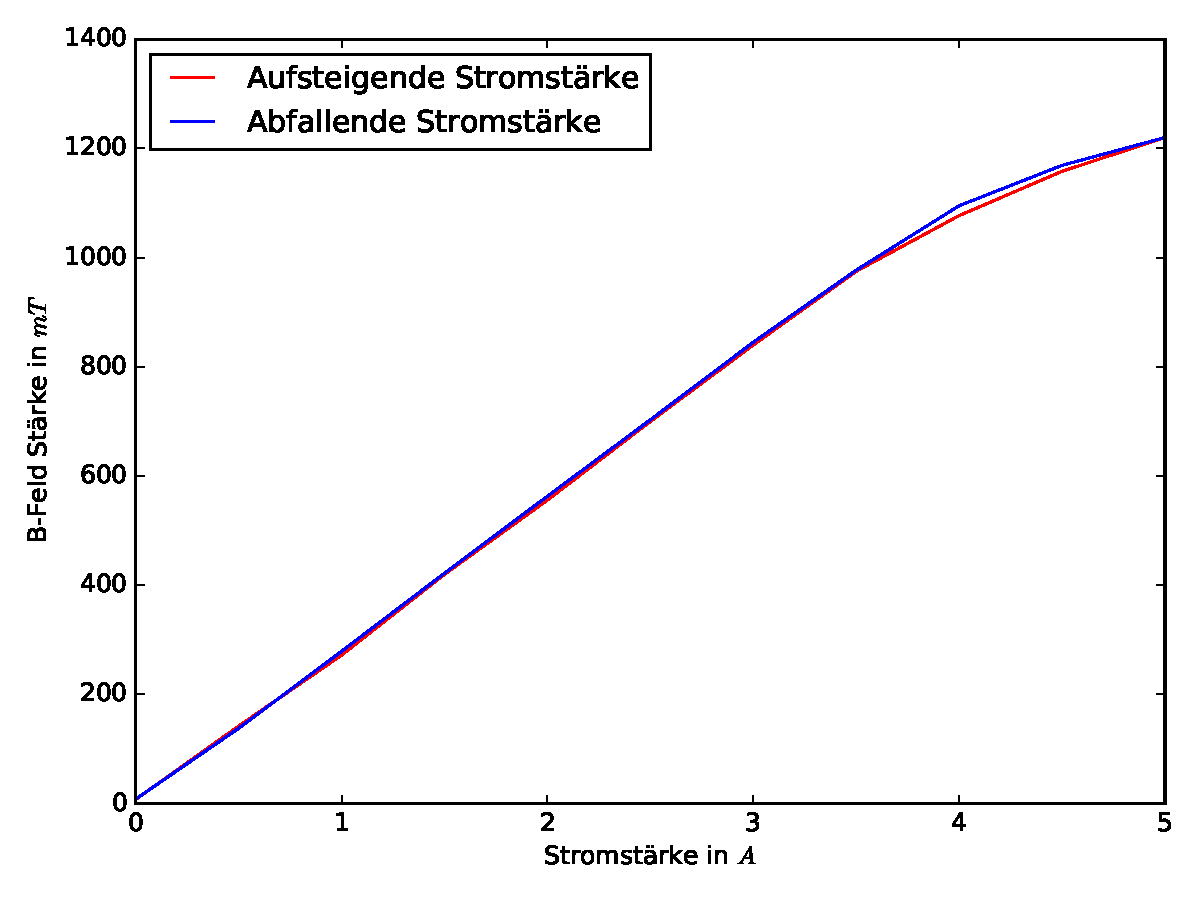
\includegraphics[width=\textwidth]{Hysterese.pdf}
  \caption{Der auftretende Hystereseeffekt}
  \label{fig:Hysterese}
\end{figure}

In dem Diagramm wird deutlich, dass sich die Verläufe der $B$-Feldstärke bei
unterschiedlich geregelter Stromstärke kaum unterscheiden. Daran ist ersichtlich,
dass der Hystereseeffekt bei der Auswertung der Messergebnisse nur einen geringen
Einfluss hat und aus diesem Grund zu vernachlässigen ist.

Bei den im Versuch angestellten Messungen wurde stets die Stromstärke hochgeregelt,
sodass die $B$-Feldstärke gegenüber des aufgedrehten Stroms verwendet wird, um
den Proportionalitätsfaktor zwischen der Stromstärke $I$ und $B$ zu ermitteln.
Der lineare Fit ist in dem folgendem Diagramm dargestellt.

\begin{figure}
  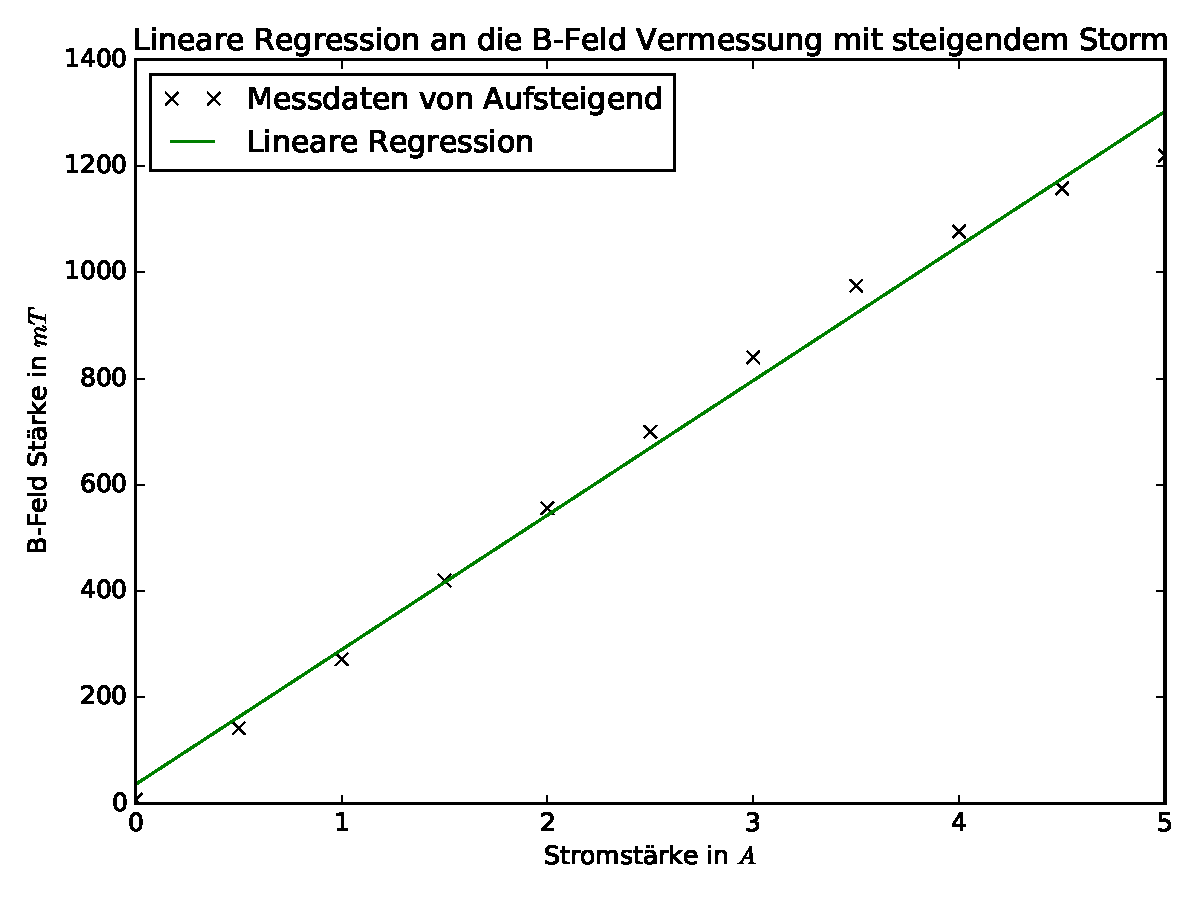
\includegraphics[width=\textwidth]{lineareRegression.pdf}
  \caption{'Lineare Regression an die $B$-Feldstärke bei aufsteigendem $I$'}
  \label{fig:lineareRegression}
\end{figure}

Als Proportionalitätsfaktor zwischen $I$ und $B$ ergibt sich somit $B =
253,35 * I$. Der Proportionalitätsfaktor wird als fehlerfrei angenommen.

\subsection{Messung der Widerstände}

Die Widerstände lassen sich über die Messergebnisse der Spannung bei variirender
Stromstärke errechnen. Das ohmsche Gesetzt besagt, dass der Widerstand der
Proportionalitätsfaktor zwischen der Spannung und der Stromstärke ist.
In dem folgenden Diagrammen ist die Spannung gegenüber der Stromstärke aufgetragen.
Die Regressionsgerade wurde direkt in Diagramme integriert.

\begin{figure}
  \includegraphics[width=\textwidth]{Widerstansmessung.pdf}
  \caption{Diagramme der Widerstandsmessung}
  \label{fig:Widerstände}
\end{figure}

Es ergibt sich für die Zinkprobe ein gemessener Widerstand von $R_Z =
(\SI{13,32\pm0,067}{\milli\ohm}$. Für die Kupferprobe ergibt sich ein gemesserner
Widerstand von $R_K = \SI{7,64\pm0,016}{\milli\ohm}$.

\subsection{Bestimmung von der Hall--Spannung $U_H$}



\section{Messergebnisse}

\subsection{Abmessungen der verwendeten Proben}

Bei der Probe Zink wurden folgende Maße genommen.
Für die Vermessung wurde eine Schieblehre verwendet.

\begin{description}
  \item[Höhe] $\SI{0,02603}{\meter}$
  \item[Breite] $\SI{0,04406}{\meter}$
  \item[Dicke] $\SI{0,00043}{\meter}$
\end{description}

Für die Probe Kupfer wurden folgenden Maße genommen.
Die Dicke der Probe wurde angegeben, die restlichen Maße wurden mit einer
Schieblehre genommen.

\begin{description}
  \item[Höhe] $\SI{0,0280}{\meter}$
  \item[Breite] $\SI{0,0253}{\meter}$
  \item[Dicke] $\SI{0,000018}{\meter}$
\end{description}

\subsection{Messung der Feldstärke bei variirendem Strom}

\floatplacement{table}{htpb}
\begin{table}
 \centering
 \label{tab:Messergebnisse_Feldstärke_Isteigt}
 \begin{tabular}[width=\textwidth]{S| S[table-format=1.1] S[table-format=3.1] S[table-format=3.0] S[table-format=3.1] S[table-format=3.0] S[table-format=3.1] S[table-format=3.0] S[table-format=3.1] S[table-format=4.0] S[table-format=4.1] S[table-format=4.0]}
     \midrule
      $I$ \text{\;in\;} \si{\ampere} & 0 & 0,5 & 1 & 1,5 & 2 & 2,5 & 3 & 3,5 & 4 & 4,5 & 5 \\
      $B$ \text{\;in\;} \si{\milli\tesla} & 7,7 & 142 & 272 & 420 & 556 & 700 & 840 & 975 & 1077 & 1158 & 1220 \\
      \bottomrule
\end{tabular}
  \caption{$B$-Feldstärke bei steigender Stromstärke}
\end{table}


\floatplacement{table}{htpb}
\begin{table}
 \centering
 \label{tab:Messergebnisse_Feldstärke_Ifällt}
 \begin{tabular}[width=\textwidth]{S| S[table-format=4.0] S[table-format=4.1] S[table-format=4.0] S[table-format=3.1] S[table-format=3.0] S[table-format=3.1] S[table-format=3.0] S[table-format=3.1] S[table-format=3.0] S[table-format=3.1] S[table-format=3.1]}

     \midrule
      $I$ \text{\;in\;} \si{\ampere} & 5 & 4,5 & 4 & 3,5 & 3 & 2,5 & 2 & 1,5 & 1 & 0,5 & 1 \\
      $B$ \text{\;in\;} \si{\milli\tesla} & 1220 & 1169 & 1095 & 977 & 845 & 703 & 563 & 422 & 279 & 138 & 8,3 \\
      \bottomrule
\end{tabular}
  \caption{$B$-Feldstärke bei fallender Stromstärke}
\end{table}
\FloatBarrier

\subsection{Messdaten für die Bestimmung der Widerstände der Proben}

\floatplacement{table}{htpb}
\begin{table}
 \centering
 \label{tab:Spannung_Zink}
 \begin{tabular}[width=\textwidth]{S| S[table-format=2.2] S[table-format=2.2] S[table-format=2.1] S[table-format=2.1] S[table-format=2.1] S[table-format=2.1] S[table-format=2.1] S[table-format=2.1] S[table-format=3.1] S[table-format=3.1] S[table-format=3.1]}

     \midrule
      $I$ \text{\;in\;} \si{\ampere} & 0 & 1 & 2 & 3 & 4 & 5 & 6 & 7 & 8 & 9 & 10 \\
      $U$ \text{\;in\;} \si{\milli\volt} & -0,02 & 14,13 & 27,7 & 41,1 & 55,5 & 68,3 & 81,5 & 94,7 & 107,1 & 120,3 & 133,7 \\
      \bottomrule
\end{tabular}
  \caption{Messdaten für die Probe Zink}
\end{table}


\floatplacement{table}{htpb}
\begin{table}
 \centering
 \label{tab:Spannung_Kupfer}
 \begin{tabular}[width=\textwidth]{S| S[table-format=1.2] S[table-format=2.2] S[table-format=2.1] S[table-format=2.1] S[table-format=2.1] S[table-format=2.1] S[table-format=2.1] S[table-format=2.1] S[table-format=3.1] S[table-format=3.1] S[table-format=3.1]}

     \midrule
      $I$ \text{\;in\;} \si{\ampere} & 0 & 1 & 2 & 3 & 4 & 5 & 6 & 7 & 8 & 9 & 10 \\
      $U$ \text{\;in\;} \si{\milli\volt} & 0 & 7,83 & 15,54 & 23,3 & 30,9 & 38,6 & 46,3 & 53,9 & 61,5 & 68,8 & 76,5\\
      \bottomrule
\end{tabular}
  \caption{Messdaten für die Probe Kupfer}
\end{table}
\FloatBarrier

\subsection{Messdaten für die gemessene Hall--Spannung bei konstantem Probenstrom}

\floatplacement{table}{htpb}
\begin{table}
 \centering
 \label{tab:Zink_U_H}
 \begin{tabular}[width=\textwidth]{S| S[table-format=1.3] S[table-format=1.3] S[table-format=1.3] S[table-format=1.3] S[table-format=1.3] S[table-format=1.3] S[table-format=1.3] S[table-format=1.3] S[table-format=1.3] S[table-format=1.3] S[table-format=1.3]}

     \midrule
      $I_{\text{\tiny{Spule}}}$ \text{\;in\;} \si{\ampere} & 0 & 0,5 & 1 & 1,5 & 2 & 2,5 & 3 & 3,5 & 4 & 4,5 & 5 \\
      $U$ \text{\;in\;} \si{\milli\volt} & 0,644 & 0,648 & 0,651 & 0,654 & 0,657 & 0,659 & 0,661 & 0,663 & 0,664 & 0,665 & 0,666\\
      \bottomrule
\end{tabular}
  \caption{Messdaten für Zink bei einem konstantem Probenstrom von $\SI{8}{\ampere}$}
\end{table}


\floatplacement{table}{htpb}
\begin{table}
 \centering
 \label{tab:Kupfer_U_H}
 \begin{tabular}[width=\textwidth]{S| S[table-format=2.3] S[table-format=1.3] S[table-format=1.3] S[table-format=1.3] S[table-format=1.3] S[table-format=1.3] S[table-format=1.3] S[table-format=1.3]}

     \midrule
      $I_{\text{\tiny{Spule}}}$ \text{\;in\;} \si{\ampere} & 0 & 0,5 & 1 & 1,5 & 2 & 2,5 & 3 & 3,5 \\
      $U$ \text{\;in\;} \si{\milli\volt} & -0,342 & -0,340 & -0,338 & -0,336 & -0,334 & -0,332 & -0,330 & -0,328 \\
      \bottomrule
\end{tabular}
  \caption{Messdaten für Kupfer bei einem konstantem Probenstrom von $\SI{10}{\ampere}$}
\end{table}
\FloatBarrier

\subsubsection{Daten nach Umpolung}

\floatplacement{table}{htpb}
\begin{table}
 \centering
 \label{tab:Zink_U_H_umgepolt}
 \begin{tabular}[width=\textwidth]{S| S[table-format=1.3] S[table-format=1.3] S[table-format=1.3] S[table-format=1.3] S[table-format=1.3] S[table-format=1.3] S[table-format=1.3] S[table-format=1.3] S[table-format=1.3] S[table-format=1.3] S[table-format=1.3]}

     \midrule
      $I_{\text{\tiny{Spule}}}$ \text{\;in\;} \si{\ampere} & 0 & 0,5 & 1 & 1,5 & 2 & 2,5 & 3 & 3,5 & 4 & 4,5 & 5 \\
      $U$ \text{\;in\;} \si{\milli\volt} & 0,647 & 0,646 & 0,645 & 0,644 & 0,642 & 0,641 & 0,639 & 0,638 & 0,636 & 0,635 & 0,634\\
      \bottomrule
\end{tabular}
  \caption{Messdaten für Zink bei einem konstantem Probenstrom von $\SI{8}{\ampere}$}
\end{table}


\floatplacement{table}{htpb}
\begin{table}
 \centering
 \label{tab:Kupfer_U_H_umgepolt}
 \begin{tabular}[width=\textwidth]{S| S[table-format=2.3] S[table-format=1.3] S[table-format=1.3] S[table-format=1.3] S[table-format=1.3] S[table-format=1.3] S[table-format=1.3] S[table-format=1.3]}

     \midrule
      $I_{\text{\tiny{Spule}}}$ \text{\;in\;} \si{\ampere} & 0 & 0,5 & 1 & 1,5 & 2 & 2,5 & 3 & 3,5\\
      $U$ \text{\;in\;} \si{\milli\volt} & -0,340 & -0,342 & -0,343 & -0,345 & -0,347 & -0,349 & -0,351 & -0,353 \\
      \bottomrule
\end{tabular}
  \caption{Messdaten für Kupfer bei einem konstantem Probenstrom von $\SI{10}{\ampere}$}
\end{table}
\FloatBarrier

\subsection{Messdaten für die gemessene Hall-Spannung bei konstantem Spulenstrom}

\floatplacement{table}{htpb}
\begin{table}
 \centering
 \label{tab:Zink_U_H_2}
 \begin{tabular}[width=\textwidth]{S| S[table-format=2.3] S[table-format=1.3] S[table-format=1.3] S[table-format=1.3] S[table-format=1.3] S[table-format=1.3] S[table-format=1.3] S[table-format=1.3] S[table-format=1.3] S[table-format=1.3]
 S[table-format=1.3]}

     \midrule
      $I_{\text{\tiny{Probe}}}$ \text{\;in\;} \si{\ampere} & 0 & 0,8 & 1,6 & 2,4 & 3,2 & 4 & 4,8 & 5,6 & 6,4 & 7,2 & 8 \\
      $U$ \text{\;in\;} \si{\milli\volt} & -0,020 & 0,045 & 0,109 & 0,174 & 0,234 & 0,304 & 0,365 & 0,431 & 0,495 & 0,560 & 0,626 \\
      \bottomrule
\end{tabular}
  \caption{Messdaten für Zink bei einem konstantem Spulenstrom von $\SI{5}{\ampere}$}
\end{table}


\floatplacement{table}{htpb}
\begin{table}
 \centering
 \label{tab:Kupfer_U_H_2}
 \begin{tabular}[width=\textwidth]{S| S[table-format=2.3] S[table-format=1.3] S[table-format=1.3] S[table-format=1.3] S[table-format=1.3] S[table-format=1.3] S[table-format=1.3] S[table-format=1.3] S[table-format=1.3] S[table-format=1.3] S[table-format=1.3]}

     \midrule
      $I_{\text{\tiny{Probe}}}$ \text{\;in\;} \si{\ampere} & 0 & 1 & 2 & 3 & 4 & 5 & 6 & 7 & 8 & 9 & 10 \\
      $U$ \text{\;in\;} \si{\milli\volt} & - 0,336 & - 0,338 & - 0,340 & - 0,342 & - 0,343 & - 0,345 & - 0,347 & - 0,348 & -0,350 & -0,351 & -0,352 \\
      \bottomrule
 \end{tabular}
  \caption{Messdaten für Kupfer bei einem konstantem Probenstrom von $\SI{3}{\ampere}$}
\end{table}
\FloatBarrier

\subsubsection{Daten nach Umpolung}

\floatplacement{table}{htpb}
\begin{table}
 \centering
 \label{tab:Zink_U_H_2_umgepolt}
 \begin{tabular}[width=\textwidth]{S| S[table-format=2.2] S[table-format=1.3] S[table-format=1.3] S[table-format=1.3] S[table-format=1.3] S[table-format=1.3] S[table-format=1.3] S[table-format=1.3] S[table-format=1.3] S[table-format=1.3] S[table-format=1.3]}
     \midrule
      $I_{\text{\tiny{Probe}}}$ \text{\;in\;} \si{\ampere} & 0 & 0,8 & 1,6 & 2,4 & 3,2 & 4 & 4,8 & 5,6 & 6,4 & 7,2 & 8 \\
      $U$ \text{\;in\;} \si{\milli\volt} & -0,020 & 0,047 & 0,116 & 0,184 & 0,250 & 0,318 & 0,389 & 0,456 & 0,527 & 0,597 & 0,666 \\
      \bottomrule
\end{tabular}
  \caption{Messdaten für Zink bei einem konstantem Spulenstrom von $\SI{5}{\ampere}$}
\end{table}


\floatplacement{table}{htpb}
\begin{table}
 \centering
 \label{tab:Kupfer_U_H_2_umgepolt}
 \begin{tabular}[width=\textwidth]{S| S[table-format=2.3] S[table-format=1.3] S[table-format=1.3] S[table-format=1.3] S[table-format=1.3] S[table-format=1.3] S[table-format=1.3] S[table-format=1.3] S[table-format=1.3] S[table-format=1.3] S[table-format=1.3]}
     \midrule
      $I_{\text{\tiny{Probe}}}$ \text{\;in\;} \si{\ampere} & 0 & 1 & 2 & 3 & 4 & 5 & 6 & 7 & 8 & 9 & 10 \\
      $U$ \text{\;in\;} \si{\milli\volt} & - 0,338  & - 0,337 & - 0,336 & - 0,335 & - 0,335 & - 0,334 & - 0,333 & - 0,332 & - 0,332 & - 0,332 & - 0,330 \\
      \bottomrule
\end{tabular}
  \caption{Messdaten für Kupfer bei einem konstantem Probenstrom von $\SI{3}{\ampere}$}
\end{table}



\end{document}
